\documentclass[
	12pt,
	a4paper,
	bibtotoc,
	cleardoubleempty, 
	idxtotoc,
	ngerman,
	openright
	final,
	listof=nochaptergap,
	]{scrbook}

\usepackage[T1]{fontenc}
\usepackage[utf8]{inputenc}
\usepackage[pdftex]{graphicx} %von EG hinzugefügt
\usepackage{float} %von EG hinzugefügt
\renewcommand{\baselinestretch}{1.5} %von EG hinzugefügt

% ##################################################
% Unterstuetzung fuer die deutsche Sprache
% ##################################################
\usepackage{ngerman}
\usepackage[ngerman]{babel}

% ##################################################
% Dokumentvariablen
% ##################################################

% Persoenliche Daten
\newcommand{\docNachnameA}{Grituc}
\newcommand{\docVornameA}{Eugeniu}
\newcommand{\docEmailA}{eugeniu.grituc@hs-furtwangen.de}
\newcommand{\docMatrikelnummerA}{250301}
\newcommand{\docNachnameB}{Halilaj}
\newcommand{\docVornameB}{Ilirian}
\newcommand{\docEmailB}{ilirian.halilaj@hs-furtwangen.de}
\newcommand{\docMatrikelnummerB}{248389}
\newcommand{\docNachnameC}{Oberhauser}
\newcommand{\docVornameC}{Jurek}
\newcommand{\docEmailC}{jurek.oberhauser@hs-furtwangen.de}
\newcommand{\docMatrikelnummerC}{----}
\newcommand{\docNachnameD}{Lang}
\newcommand{\docVornameD}{Maximilian}
\newcommand{\docEmailD}{m.lang@hs-furtwangen.de}
\newcommand{\docMatrikelnummerD}{205853}
\newcommand{\docNachnameE}{Kotzjan}
\newcommand{\docVornameE}{Michael}
\newcommand{\docEmailE}{michael.kotzjan@hs-furtwangen.de}
\newcommand{\docMatrikelnummerE}{250855}

% Dokumentdaten
\newcommand{\docTitle}{FHFTrain}
%\newcommand{\docUntertitle}{} % Kein Untertitel
\newcommand{\docUntertitle}{Simulation eines Zugbetriebes mit Bahnhöfen}
% Arten der Arbeit: Bachelorthesis, Masterthesis, Seminararbeit, Diplomarbeit
\newcommand{\docArtDerArbeit}{Semesterprojekt}
%Studiengaenge: Allgemeine Informatik Bachelor, Computer Networking Bachelor,
% Software-Produktmanagement Bachelor, Advanced Computer Scinece Master
\newcommand{\docStudiengang}{Allgemeine Informatik}
\newcommand{\docAbgabedatum}{----}
\newcommand{\docErsterReferent}{Prof. Dr. Rainer Müller}

% ##################################################
% Allgemeine Pakete
% ##################################################

% Abbildungen einbinden
\usepackage{graphicx}

% Zusaetsliche Sonderzeichen
\usepackage{dingbat}

% Farben
\usepackage{color}
\usepackage[usenames,dvipsnames,svgnames,table]{xcolor}

% Maskierung von URLs und Dateipfaden
\usepackage[hyphens]{url}

% Deutsche Anfuehrungszeichen
\usepackage[babel, german=quotes]{csquotes}

% Pakte zur Index-Erstellung (Schlagwortverzeichnis)
\usepackage{index}
\makeindex

% Ipsum Lorem
% Paket wird nur für das Beispiel gebraucht und kann gelöscht werden
\usepackage{lipsum}

% ##################################################
% Seitenformatierung
% ##################################################
\usepackage[
	portrait,
	bindingoffset=1.5cm,
	inner=2.5cm,
	outer=2.5cm,
	top=3cm,
	bottom=2cm,
	%includeheadfoot
	]{geometry}

% ##################################################
% Kopf- und Fusszeile
% ##################################################

\usepackage{fancyhdr}

\pagestyle{fancy}
\fancyhf{}
\fancyhead[EL,OR]{\sffamily\thepage}
\fancyhead[ER,OL]{\sffamily\leftmark}

\fancypagestyle{headings}{}

\fancypagestyle{plain}{}

\fancypagestyle{empty}{
  \fancyhf{}
  \renewcommand{\headrulewidth}{0pt}
}

%Kein "Kapitel # NAME" in der Kopfzeile
\renewcommand{\chaptermark}[1]{
	\markboth{#1}{}
   	\markboth{\thechapter.\ #1}{}
}

% ##################################################
% Schriften
% ##################################################

% Stdandardschrift festlegen
\renewcommand{\familydefault}{\sfdefault}

% Standard Zeilenabstand: 1,5 zeilig
\usepackage{setspace}
\onehalfspacing 

% Schriftgroessen festlegen
\addtokomafont{chapter}{\sffamily\large\bfseries} 
\addtokomafont{section}{\sffamily\normalsize\bfseries} 
\addtokomafont{subsection}{\sffamily\normalsize\mdseries} 
\addtokomafont{caption}{\sffamily\normalsize\mdseries} 

% ##################################################
% Inhaltsverzeichnis / Allgemeine Verzeichniseinstellungen
% ##################################################

\usepackage{tocloft}

% Punkte auch bei Kapiteln
\renewcommand{\cftchapdotsep}{3}
\renewcommand{\cftdotsep}{3}

% Schriftart und -groesse im Inhaltsverzeichnis anpassen
\renewcommand{\cftchapfont}{\sffamily\normalsize}
\renewcommand{\cftsecfont}{\sffamily\normalsize}
\renewcommand{\cftsubsecfont}{\sffamily\normalsize}
\renewcommand{\cftchappagefont}{\sffamily\normalsize}
\renewcommand{\cftsecpagefont}{\sffamily\normalsize}
\renewcommand{\cftsubsecpagefont}{\sffamily\normalsize}

%Zeilenabstand in den Verzeichnissen einstellen
\setlength{\cftparskip}{.5\baselineskip}
\setlength{\cftbeforechapskip}{.1\baselineskip}

% ##################################################
% Abbildungsverzeichnis und Abbildungen
% ##################################################

\usepackage{caption}

\usepackage{wrapfig}

% Nummerierung von Abbildungen
\renewcommand{\thefigure}{\arabic{figure}}
\usepackage{chngcntr}
\counterwithout{figure}{chapter}

% Abbildungsverzeichnis anpassen
\renewcommand{\cftfigpresnum}{Abbildung }
\renewcommand{\cftfigaftersnum}{:}

% Breite des Nummerierungsbereiches [Abbildung 1:]
\newlength{\figureLength}
\settowidth{\figureLength}{\bfseries\cftfigpresnum\cftfigaftersnum}
\setlength{\cftfignumwidth}{\figureLength}
\setlength{\cftfigindent}{0cm}

% Schriftart anpassen
\renewcommand\cftfigfont{\sffamily}
\renewcommand\cftfigpagefont{\sffamily}

% ##################################################
% Tabellenverzeichnis und Tabellen
% ##################################################

% Nummerierung von Tabellen
\renewcommand{\thetable}{\arabic{table}}
\counterwithout{table}{chapter}

% Tabellenverzeichnis anpassen
\renewcommand{\cfttabpresnum}{Tabelle }
\renewcommand{\cfttabaftersnum}{:}

% Breite des Nummerierungsbereiches [Abbildung 1:]
\newlength{\tableLength}
\settowidth{\tableLength}{\bfseries\cfttabpresnum\cfttabaftersnum}
\setlength{\cfttabnumwidth}{\tableLength}
\setlength{\cfttabindent}{0cm}

%Schriftart anpassen
\renewcommand\cfttabfont{\sffamily}
\renewcommand\cfttabpagefont{\sffamily}

% Unterdrueckung von vertikalen Linien
\usepackage{booktabs}

% ##################################################
% Listings (Quellcode)
% ##################################################

\usepackage{listings}
\lstset{
	language=c++,
	backgroundcolor=\color{white},
	breaklines=true,
	prebreak={\carriagereturn},
 	breakautoindent=true,
 	numbers=left,
 	numberstyle=\tiny,
 	stepnumber=1,
 	numbersep=5pt,
 	showstringspaces=true,
 	keywordstyle=\color{blue},
   	commentstyle=\color{green},   
   	stringstyle=\color{gray}
}
  	
% ##################################################
% Theoreme
% ##################################################
  	
% Umgebung fuer Beispiele
\newtheorem{beispiel}{Beispiel}

% Umgebung fuer These
\newtheorem{these}{These}

% Umgebung fuer Definitionen
\newtheorem{definition}{Definition}
  	
% ##################################################
% Literaturverzeichnis
% ##################################################

\usepackage{bibgerm}

% ##################################################
% Abkuerzungsverzeichnis
% ##################################################

\usepackage[printonlyused]{acronym}

% ##################################################
% PDF / Dokumenteninternelinks
% ##################################################

\usepackage[
	colorlinks=false,
   	linkcolor=black,
   	citecolor=black,
  	filecolor=black,
	urlcolor=black,
    bookmarks=true,
    bookmarksopen=true,
    bookmarksopenlevel=3,
    bookmarksnumbered,
    plainpages=false,
    pdfpagelabels=true,
    hyperfootnotes,
    pdftitle ={\docTitle},
    pdfauthor={\docNachnameA,~\docNachnameB,~\docNachnameC,~\docNachnameD,~\docNachnameE},
    pdfcreator={\docNachnameA,~\docNachnameB,~\docNachnameC,~\docNachnameD,~\docNachnameE}]{hyperref}


\begin{document}

\setcounter{secnumdepth}{3}

% Titelblatt
\begin{titlepage}
\pagestyle{empty}

% ##################################################
% HFU-Logo einbinden
% ##################################################
\begin{flushright}
\begin{figure}[ht]
\flushright

\includegraphics[height=3cm]{content/pictures/hfu.jpg}
\end{figure}
\end{flushright}

% ##################################################
% Titel
% ##################################################
\begin{center}
{\fontsize{18}{22} \selectfont \docArtDerArbeit}\\[5mm]
{\fontsize{18}{22} \selectfont im Studiengang} \\[5mm]
{\fontsize{18}{22} \selectfont \docStudiengang}\\
\vspace{1cm}
\begin{onehalfspace}
{\fontsize{22}{26} \selectfont \textbf{\docTitle}}\\[5mm]
{\fontsize{18}{22} \selectfont \docUntertitle}


\end{onehalfspace}
\end{center}

% ##################################################
% Zusatzinformationen
% ##################################################
\vfill
\begin{center}
\begin{tabular}{lcl}
Referent		&:& \docErsterReferent \\	
Vorgelegt am 	&:& \docAbgabedatum 	\\
Vorgelegt von 	&:& \docVornameA~\docNachnameA~(Mtr.-Nr. \docMatrikelnummerA)\\
				& & \docEmailA\\
				& & \docVornameB~\docNachnameB~(Mtr.-Nr. \docMatrikelnummerB)\\
				& & \docEmailB\\
				& & \docVornameC~\docNachnameC~(Mtr.-Nr. \docMatrikelnummerC)\\
				& & \docEmailC\\
				& & \docVornameD~\docNachnameD~(Mtr.-Nr. \docMatrikelnummerD)\\
				& & \docEmailD\\
				& & \docVornameE~\docNachnameE~(Mtr.-Nr. \docMatrikelnummerE)\\
				& & \docEmailE\\			
\end{tabular}
\end{center}
\end{titlepage}
\cleardoubleemptypage

\frontmatter

% Inhaltsverzeichnis
\tableofcontents
\addcontentsline{toc}{chapter}{Inhaltsverzeichnis}
\cleardoubleemptypage

% Abbildungsverzeichnis einbinden und ins Inhaltsverzeichnis
% WORKAROUND: tocloft und KOMA funktionieren zusammen nicht
% korrekt\phantomsection
\addcontentsline{toc}{chapter}{\listfigurename} 
\listoffigures
\cleardoubleemptypage

% Tabellenverzeichnis einbinden und ins Inhaltsverzeichnis
% WORKAROUND: tocloft und KOMA funktionieren zusammen nicht
% korrekt\phantomsection
\phantomsection
\addcontentsline{toc}{chapter}{\listtablename}
\listoftables
\cleardoubleemptypage

% Abkürzungsverzeichnis
\chapter*{Abkürzungsverzeichnis\markboth{Abkürzungsverzeichnis}{}}
\addcontentsline{toc}{chapter}{Abkürzungsverzeichnis}

\begin{acronym}
\acro{HFU}{Hochschule Furtwangen University}
\end{acronym}

\mainmatter

% Unsere Kapitel
\chapter{Einleitung}

Im Gegensatz zu den meisten anderen Semesterprojekten stand bei unserem Projekt nicht im Vorraus was gemacht werden sollte und was das Ziel war, diese Entscheidung mussten wir selber fällen.\\
Dementsprechend startete das Semesterprojekt denkbar undefiniert. Schon in der Projektbeschreibung war angegeben, dass es viele Möglichkeiten gibt mit der vorhandenen Soft- und Hardware ein Semesterprojekt aufzustellen. Nach einer allgemeinen Einführung mussten wir uns also überlegen, was wir dieses Semester erarbeiten wollen. Wir wussten also ungefähr zu was der Zug in der Lage war und hatten jetzt die Möglichkeit dies zu erweitern.\\
Schnell kam die Überlegung auf, ob wir den Zug nicht mithilfe eines externen Gerätes steuern könnten, der die Position des Zugs kennt und mithilfe eines Steuer-Algorithmus den optimalen Weg für den Zug festlegen kann. Hier hofften wir viel Gelerntes anwenden zu können und ein Spannendes und auch Anspruchsvolles Projekt geschaffen zu haben. So legten wir uns also darauf fest, eine externe Zugsteuerung zu entwerfen.\\
Man kann sich jetzt fragen, was der optimale Weg für einen Zug sei. Wir haben festgelegt, dass es sich um einen Personenzug handeln soll, welcher möglichst effektiv Personen von bestimmten Startbahnhöfen zum jeweiligen Zielbahnhof einer Person bringen muss. Dabei soll der Zug immer den bestmöglichen Weg wählen und auch nur anhalten, wenn wirklich Personen ein- oder aussteigen wollen.\\
Durch das Benutzen eines externen Gerätes entstanden natürlich weitere Anforderungen, die wir beachten mussten:
\begin{itemize}
	\item Wie können die beiden Geräte miteinander kommunizieren?
	\item Wie können wir mit IBM Rhapsody, der Entwicklungsumgebung, welche wir benutzten, sowohl für den Zug als auch für die externe Steuereinheit kompilieren?
	\item Was muss der Zug genau können und was die externe Steuereinheit?
\end{itemize}
Ein weiterer wichtiger Punkt war, dass wir kein jungfräuliches Projekt vor uns hatten, sondern unser Projekt auf Vorgängerprojekten der letzten Semester basierte, wir also schon definierte Hardware hatten und dementsprechend auch dazugehörige Software.\\ 
In dieser Dokumentation werden, nebst einer allgemeinen Projektbeschreibung, die einzelnen Arbeitspakete aufgeführt, die in dem Projekt bearbeitet wurden.

\chapter{Projektbeschreibung}

Das Projekt wurde in zwei Versionen aufgeteilt, von denen zeitlich nur die erste umgesetzt werden konnte.

\section{Erste Version}

In der ersten Version des Semesterprojektes werden grundlegende Funktionen umgesetzt. Geplant ist ein Transportszenario mit vier Bahnhöfen (Siehe Abbildung \ref{pic:route} aus Kapitel Algorithmus).\\
Auf dieser Strecke fährt ein Zug ohne Anhänger, auf welchem ein Embedded Linux läuft. Der Zug erhält Anweisungen von einer Zentralsteuerung, einem Raspberry Pi, und gibt an diese seine Position durch. Die Kommunikation erfolgt mittels einer Socket Verbindung. Der Pi und der Zug befinden sich im gleichen Netzwerk. Weiterhin werden Virtuelle Fahrgäste in den Bahnhöfen angelegt, welche vom Zug abgeholt werden sollen. Jeder Passagier möchte möglichst schnell zu einem bestimmten Bahnhof gebracht werden. Der Zielbahnhof wird für jeden Passagier abgelegt. Die Erstellung der Fahrgäste erfolgt durch Eingabe eines Szenarios per Kommandozeile in die Zentralsteuerung.\\
In diesem ersten Szenario werden die Weichen nicht benutzt. Somit erfolgt die Verteilung der Bahnhöfe ausschließlich auf der äußeren Bahn. Es existieren weitere wichtige Punkte zwischen den Bahnhöfen. Bahnhöfe und diese weiteren Punkte sind physisch gesehen nur RFID-Tags, die der Zug beim Überfahren lesen kann.\\
Eine Unterscheidung, ob es sich bei einem Tag um einen Bahnhof oder einen anderen Punkt handelt, erfolgt nur durch die Zentrale Steuereinheit.

\section{Zweite Version}

In der zweiten Version besitzt unser Bahnhofssystem mehr Bahnhöfe, wodurch die Weichen ebenfalls angesteuert werden müssen. Dies geschieht mittels eines separaten Java Programmes, da Java hier bessere Funktionen bietet.\\
Um einen Korrekten Ablauf zu gewährleisten bekommt der Zug seine Anweisung erst gesendet wenn die Strecke frei ist, also alle Weichen, die für diesen Befehl benötigt werden, richtig gesetzt wurden.\\
Nach dem Setzen einer Weiche wird überprüft, ob diese sich in der Korrekten Position befindet.\\
Unterscheiden soll sich auch die Generierung von Passagieren. In unserer ersten Version wurden diese noch von der Zentralsteuerung einmalig generiert. Nun möchten wir dem Besucher unserer Anlage die Möglichkeit geben selbst Passagiere an Bahnhöfen zu platzieren. Dazu stellen wir ein Webinterface zur Verfügung. Die Anzahl der Passagiere wird gespeichert und kann von der Zentralsteuerung zur Berücksichtigung bei der Erstellung neuer Anweisungen ausgelesen werden.\\
Zusätzlich muss über das Webinterface angegeben werden, zu welchem Bahnhof die Passagiere möchten. Dies soll jederzeit möglich sein, der Pi soll dann auf die Eingaben möglichst schnell reagieren und dem Zug, wenn nötig, neue Befehle übermitteln.

\chapter{Architektur}
Nachdem wir unser Projektziel für uns gesetzt hatten mussten wir schauen wie das sich realisieren lässt. Als erstes einigten wir uns darauf das wir einen Raspberry Pi für die externe Zugsteuerung benutzen. Dann mussten wir uns überlegen wie wir den Zug mit dem Raspberry Pi kommunizieren lassen, damit diese Information zwischen einander austauschen können. Bevor wir das aber entscheiden konnten mussten wir erst die folgenden Fragen beantworten:
\begin{itemize}
\item Was muss der Zug können?
\item Was der Raspberry Pi?
\item Welche Informationen müssen übertragen werden? 
\end{itemize}
Zuerst haben wir uns überlegt, was der Zug können muss, was grob gesagt nur das Transportieren von Fahrgästen von einem Bahnhof zu einem anderen Bahnhof ist. Daraus konnten wir ableiten, dass die Erkennung seiner aktuellen Position eine der wichtigsten Aufgaben des Zuges ist, denn wenn wir nicht wissen wo der Zug ist, dann können wir ihm auch nicht sagen, wo er hinfahren soll. Des weiteren muss der Zug einstellen können, wie schnell er fährt, und Information übermitteln können. Damit hatten wir den ersten Entwurf der Funktionalität des Zuges bestimmt und konnten uns dem Raspberry Pi zuwenden. Dieser muss als eine externe Steuereinheit bestimmen, welchen Weg der Zug fahren soll. Dazu braucht er die Informationen über die Position des Zuges und an welchem Bahnhof Personen stehen und wohin diese gehen wollen. Des weiteren muss er dann noch dem Zug übermitteln können wohin er als nächstes fahren soll. Mit unseren Überlegungen hatten wir schon automatisch unsere dritte Frage beantwortet. Denn der Zug muss dem Raspberry Pi seine aktuelle Position übermitteln und der Raspberry Pi muss dem Zug einen Befehl schicken wohin und mit welcher Geschwindigkeit er als nächstes fahren soll. 

Nach dem wir unsere Fragen beantwortet hatten, wollten wir versuch diese mit Hilfe eines Klassendiagramms zu konkretisieren (Siehe Abbildung \ref{pic:ClassDiagram}).In nachfolgenden sind alle Klassen die Thread in ihrem Namen haben auch Threads. Die Klasse LocateThread in der Train-Komponente des Klassendiagramms beschäftigt sich ausschließlich mit der Bestimmung der Position des Zuges. Zur Bestimmung der Position  haben wir auf der Strecke RFID-Tags verteilt die der LocateThread vom Zug beim Überfahren lesen kann und danach sie weiter an die Klasse TrainSpeakerThread schickt. Dieser vergleicht nach erhalten der Position diese mit der eingetragenen Position in der Klasse Order. Falls die Positionen sich unterscheiden ist entweder etwas schiefgelaufen oder der Zug ist gerade erst angefahren und hat zum ersten mal seine Position bestimmt. Bei beiden Fällen wird die Geschwindigkeit des Zugs auf 0 gesetzt und er wartet somit auf weitere Befehle. Falls die Positionen gleich sind wird die afterSpeed Geschwindigkeit aus der Klasse Order genommen und dem TrainThread übermittel, welcher dann diese Geschwindigkeit setzt. Als letztes schickt der TrainSpeakerThread über eine Socket-Verbindung die Position des Zuges an den Raspberry Pi. Diese Nachricht kommt dann an die Klasse PiListenerThread, welcher diese in der Klasse TrainStatus abspeichert. Danach kann die Klasse PiAlgorithm, welche auch ein Thread ist, durch die aktuelle Position des Zugs aus dem TrainStatus auslesen und schauen wohin der Zug als nächstes fahren soll(genaueres wir im Kapitel Algorithm erklärt). Diesen Befehl schickt er an den PiSpeakerThread, welcher diesen weiter über die Socket-Verbindung schickt. Der Befehl wird vom TrainListenerThread erhalten, welcher den Befehl in der Klasse Order speichert. Zuletzt wird noch die beforeSpeed Geschwindigkeit die im Befehl enthalten ist an den TrainThread übermittelt, welcher dann die Geschwindigkeit des Zuges darauf setzt. Damit hätte man einen gesamten Durchlauf gemacht, welcher wieder von neuen beginnt wenn der Zug eine neue Position liest.  


\begin{figure}[H]	
\caption{Klassendiagramm}
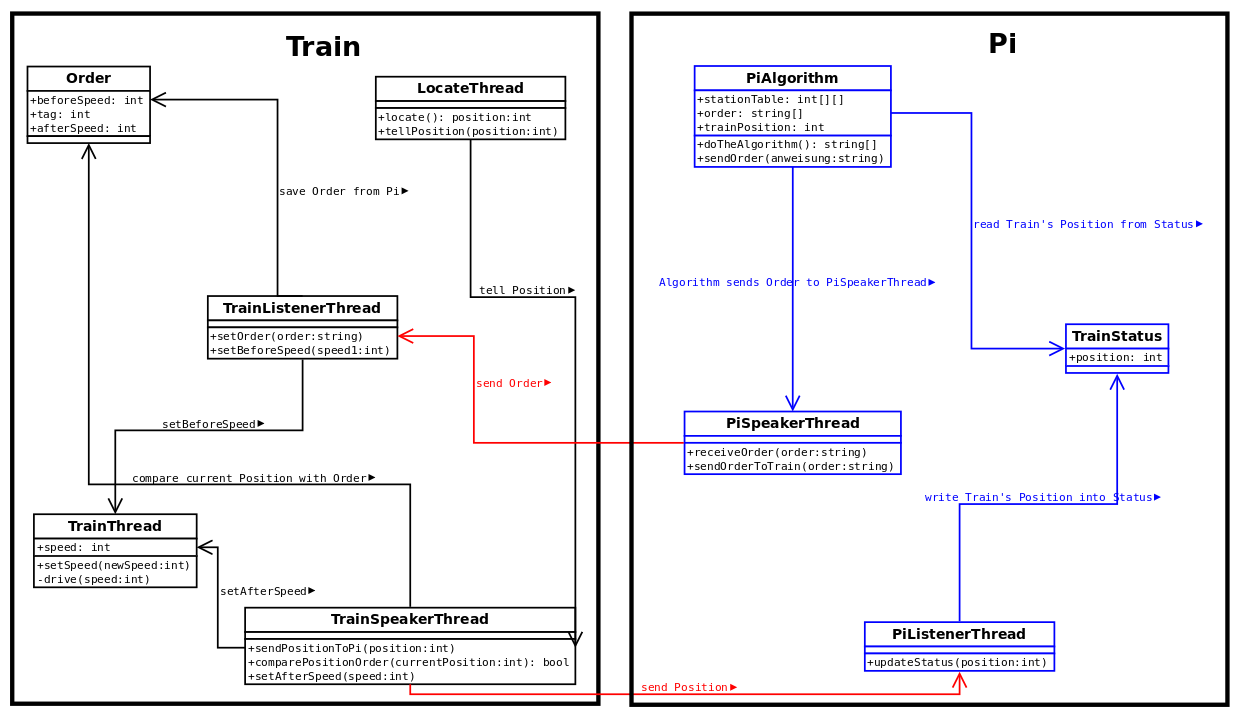
\includegraphics[width=2\textwidth, width=465pt]{content/images/ClassDiagram.png}
\label{pic:ClassDiagram}
\end{figure}



\begin{figure}[H]	
\caption{Use Case Diagramm}
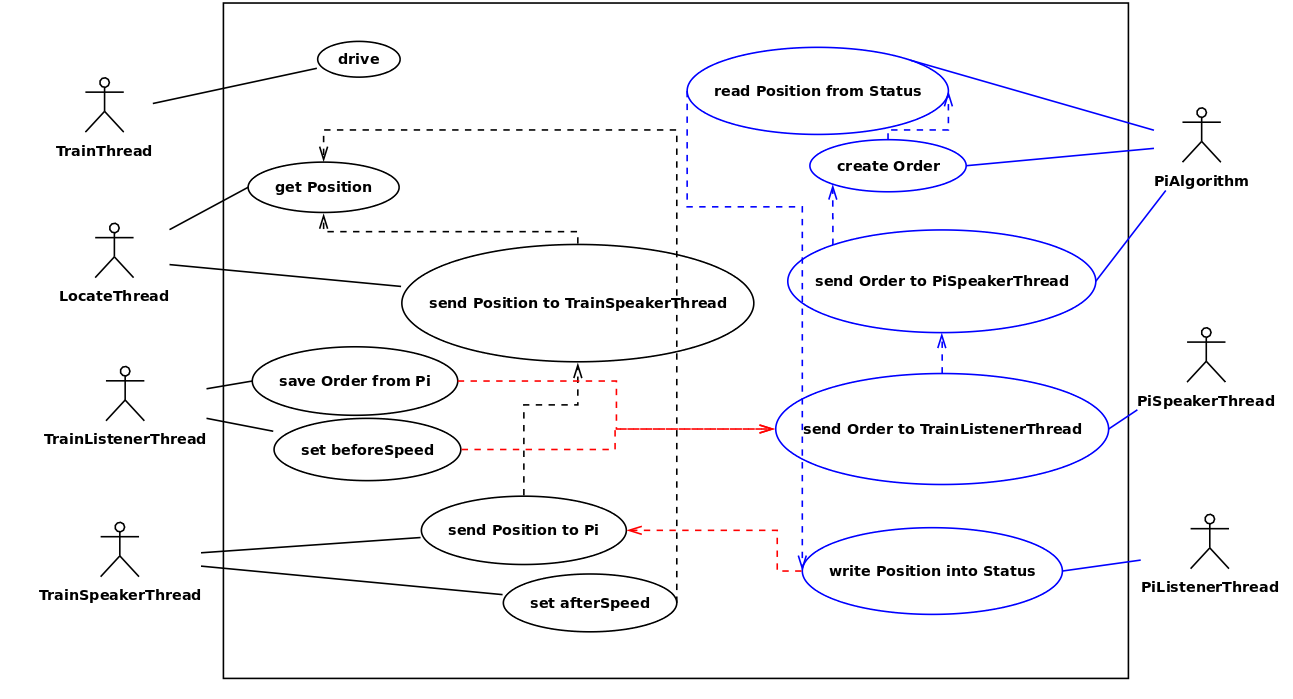
\includegraphics[width=2\textwidth, width=465pt]{content/images/UseCaseDia.png}
\label{pic:UseCaseDiagram}
\end{figure}

%\chapter{Algorithmus} %wurde von EG durch content/alg ersetzt
%\documentclass[
%	12pt,
%	a4paper,
%	bibtotoc,
%	cleardoubleempty, 
%	idxtotoc,
%	ngerman,
%	openright
%	final,
%	listof=nochaptergap,
%	]{scrbook}
\renewcommand{\baselinestretch}{1.5} 
%\usepackage[T1]{fontenc}
%\usepackage[utf8]{inputenc}
%\usepackage[pdftex]{graphicx}
%\usepackage{float}
%\begin{document}

\chapter{Algorithmus}
\section{Was macht der Algorithmus?}
Der Algorithmus läuft auf dem Raspberry Pi in einem eigenen Thread. Seine Aufgabe ist es, die Route des Zuges anhand der Eingabe zu berechnen, eine Folge von Anweisungen für den Zug zu erstellen und diese eine nach der anderen dem Zug über Socket-Kanal mithilfe vom Speaker Thread mitzuteilen. Eine weitere Aufgabe des Algorithmus ist es, die aktuelle Position des Zuges nach jeder Änderung während der Fahrt zu ermitteln und danach zu überprüfen, ob es Abweichungen von der geplannten Strecke gibt. Solche Anweisungen muss der Algorithmus berücksichtigen und entsprechend handeln, in dem er die Strecke anpasst, falls notwendig, und eine neue Folge von Anweisungen erstellt.\\
\section{Definitionen der Schlüsselwörter}
\label{chap:alg_keywords}
\textit{\textbf{Bahnhof, Zwischenhaltestelle, Position des Zuges}}: Sowohl ein Bahnhof, als auch eine Zwischenhaltestelle entsprechen einem (aus 8 im Projekt vorhandenen) RFID-Tag, den der Zug erkennen kann und wessen "Name" (und somit seine Position) der Zug dem Pi mitteilt. Ein Bahnhof wird von einer Zwischenhaltestelle dadurch unterschieden, dass auf einem Bahnhof ein sinnvolles Anhalten stattfinden kann: Damit der Zug Reisende aufnimmt bzw. ihnen die Möglichkeit gibt, auszusteigen. Aus Bequemlichkeit sind die Bahnhöfe im Bereich [0, 3] mit natürlichen Zahlen durchnummeriert (dadurch kann man die entsprechende Zeile bzw. Spalte in der Matrix ansprechen), während die Zwischenhaltestellen 0.5, 1.5 usw. heißen. Die Zwischenhaltestellen sind lediglich für die Anweisungen, die der Pi erstellt, notwendig: Der Zug wird seine Geschwindigkeit bei einer Zwischenhaltestelle runtersetzen, falls er bei dem folgenden Bahnhof anhalten muss. Außerdem könnte man diese Zwischenhaltestelle für eine niedrigere Geschwindigkeit bei gefährlichen Kurwen verwenden: Bei manchen Zwischenhaltestellen festlegen, dass der Zug dort immer langsam fahren muss.\\
\\
Dabei ist es zu beachten, dass die Zahlen 0.5, 1.5 usw. vom Typ double sind. Zwei double Werte soll man aufgrund der Rundungsfehler und der eingeschränkten Genauigkeit nie vergleichen: Die Gleitkommazahlen, die auf dem Papier gleich sind, werden auf verschiedenen Geräten unterschiedlich dargestellt. So könnte eine Zahl 0.125 auf dem Gerät-1 binär anders aussehen, als dieselbe Zahl auf dem Gerät-2. Das Problem läßt sich allerdings durch Mapping lösen (man kann zum Beispiel mit integer Werten arbeiten und 0, 5, 10, 15, usw. anstatt 0, 0.5, 1, 1.5, usw. verwenden). In dieser Dokumentation werden die Stationen deshalb aus Bequemlichkeit weiter als 0, 0.5, 1, 1.5 usw. bezeichnet. Dies erleichtet auch die Arithmetik bei der Hauptaufgabe des Algorithmus, nämlich bei der Erstellung der Anweisungen. Weitere Information darüber findet man in der Beschreibung der \textit{createOrderlist()} - Methode.\\
\begin{figure}[H]	
\caption{Route (Fahrt im Uhrzeigersinn)}
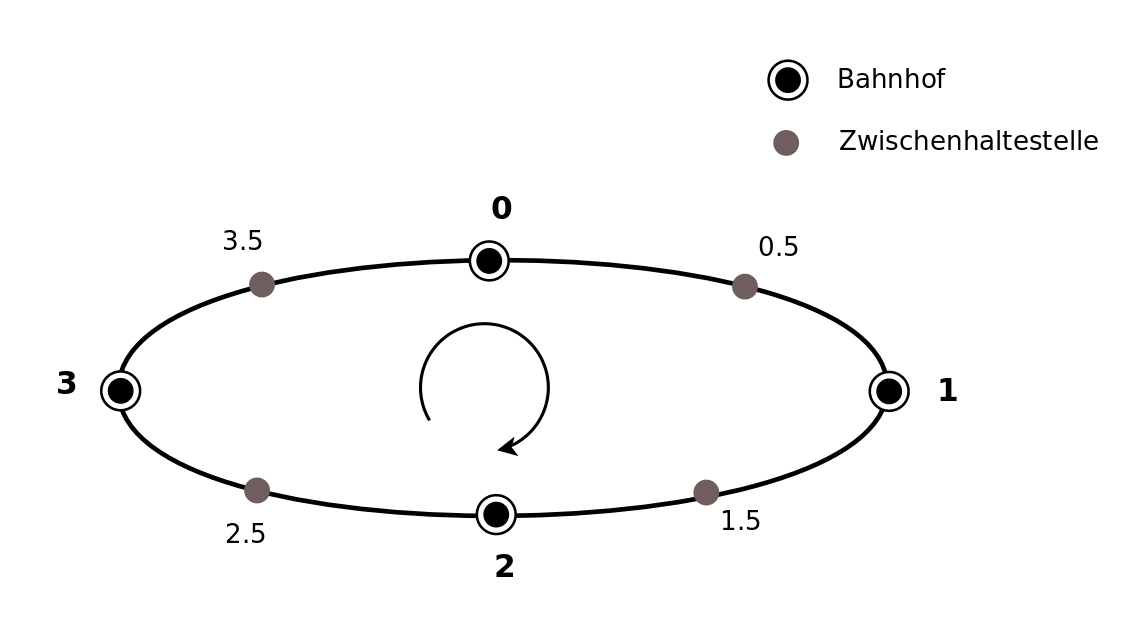
\includegraphics[width=2\textwidth, width=470pt]{content/images/route.png}
\label{pic:route}
\end{figure}
\noindent
\textit{\textbf{Start-Bahnhof}}: Dies ist der Bahnhof, an dem der Zug nach dem Start des System ankommt. Diese Position wird auch als erste dem Algorithmus auf der Pi-Seite mitgeteilt.\\
\\
\textit{\textbf{Anweisung}}: Eine Anweisung besteht aus drei Teilen: einer Vor-Geschwindigkeit (weiter hier VG, im Code das Attribut \textit{beforeSpeed}), einem Tag, und einer Nach-Geschwindigkeit (weiter hier NG, im Code das Attribut \textit{afterSpeed}). Die VG wird auf der Zug-Seite sofort nach dem Eingang der Anweisung als die aktuelle Geschwindigkeit des Zuges gesetzt. Sowohl der Tag, als auch die NG werden auf der Zug-Seite temporär gespeichert. Nachdem der Zug eine Zeit gefahren ist und ein neuer Tag erkannt wurde, wird der Wert des ermittelten Tags mit dem gespeicherten Tag verglichen. So erkennt man eine Abweichung im Verhalten des Zuges. Falls keine Abweichung gibt und der erwartete Tag ermittelt wurde, wird die NG als aktuelle Geschwindigkeit gesetzt und die Position (der Tag) des Zuges wird dem Pi mitgeteilt.\\ 
\\
\textit{Beispiel-Anweisungen:} (2,0.5,1): "Fahre mit Geschwindigkeit 2 bis zum Tag 0.5, danach setze die Geschwindigkeit auf 1". Der erste Wert - 2 - wird danach (auf der Zug-Seite) auf eine schnelle Geschwindigkeit abgebildet, der letzte - 1 - auf eine langsame Geschwindigkeit.\\
(1,1,0): "Fahre mit Geschwindigkeit 1 bis zum Tag 1, danach setze die Geschwindigkeit auf 0". Bei Geschwindigkeit gleich 0 hält der Zug an.\\
\begin{figure}[H]	
\caption{Anweisung}
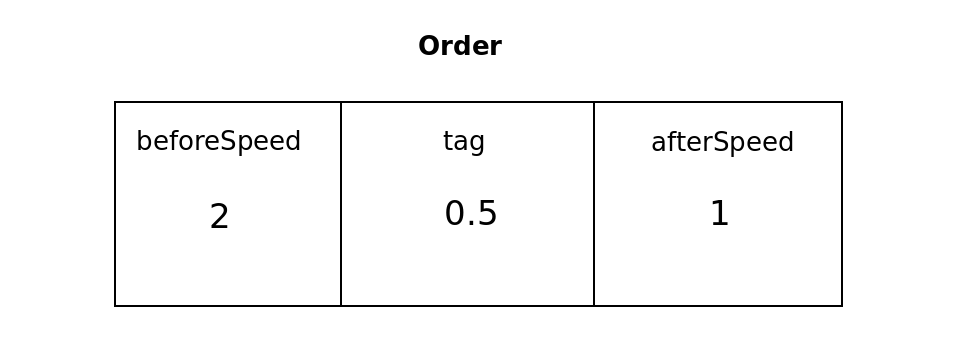
\includegraphics[width=2\textwidth, width=330pt]{content/images/order.png}
\label{pic:anweisung}
\end{figure}
\noindent
%
\section{Detaillierte Beschreibung/Ablauf}
Der Grund dafür, dass der Algorithmus in einem eigenen Thread läuft, besteht darin, dass Raspberry Pi gleichzeitig in der Lage sein muss, mit dem Zug zu kommunizieren. Dies geschieht über Socket-Kommunikation, für welche Listener und Speaker Threads auf der Pi-Seite verantwortlich sind, die ensprechend die Informationen vom Zug erhalten (nämlich die Position des Zuges, das macht Listener Thread vom Pi) und Daten dem Zug mitteilen (nämlich die neue Anweisung, das macht Speaker Thread vom Pi). \\
%
\begin{figure}[H]	
\caption{Kommunikation zwischen dem Zug und dem Raspberry Pi}
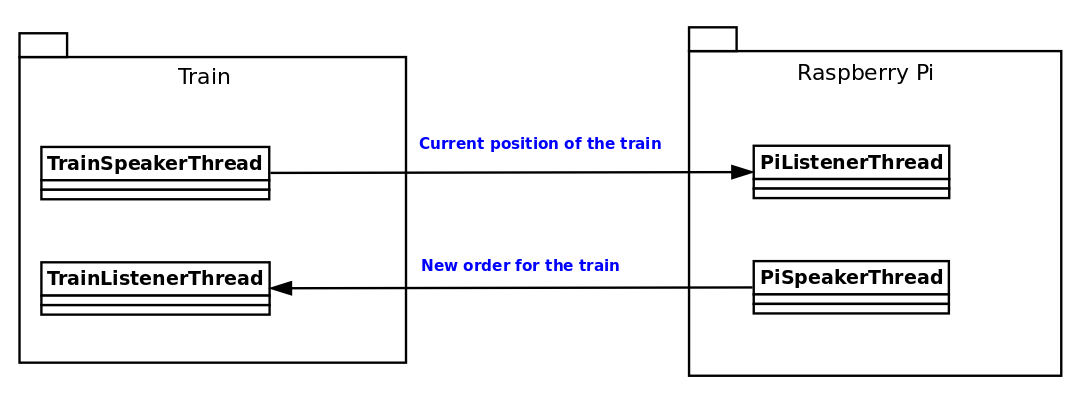
\includegraphics[width=2\textwidth, width=470pt]{content/images/communication.png}
\label{pic:communication}
\end{figure}
\noindent
Die Eingabe, die der Algorithmus bearbeiten muss, beinhaltet die Information über die Anzahl der Reisenden, ihren Abfahrtbahnhof und ihren Zielbahnhof. Dies kann für Bequemlichkeit in der Form einer Matrix gespeichert werden:\\
\\
\\
\begin{table}[H]
\caption{Szenario 1}
\center
 \begin{tabular}{|c|c|c|c|c|}
 \hline
  Von/Nach & B0 & B1 & B2 & B3 \\ \hline
  B0 & 0 & 0 & 3 & 0\\   \hline
    B1 & 0 & 0 & 0 & 7 \\   \hline
      B2 & 0 & 0 & 0 & 0\\   \hline
        B3 & 0 & 0 & 2 & 0 \\   \hline
 \end{tabular}
\end{table}
\noindent
\\
Die oben angegebene Tabelle ist folgend zu verstehen:\\
\\
- 3 Reisende wollen vom Bahnhof0 zum Bahnhof2 fahren\\
- 7 Reisende wollen vom Bahnhof1 zum Bahnhof3 fahren\\
- 2 Reisende wollen vom Bahnhof3 zum Bahnhof2 fahren\\

\begin{figure}[H]	
\caption{Szenario 1}
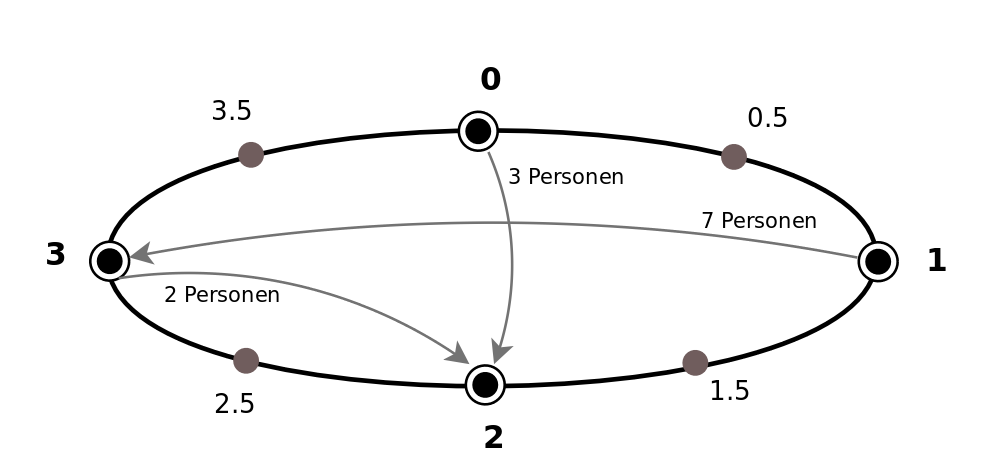
\includegraphics[width=2\textwidth, width=470pt]{content/images/szenario1.png}
\label{pic:szenario1}
\end{figure}


\section{Zusammenhang von den Methoden des Threads PiAlgorithm}
%Ablauf seiner Arbeit
Bevor man Anweisungen für den Zug erstellt, ist es sinnvoll zu wissen, wo der Zug sich befindet (die ursprüngliche Position beim Anschalten). Im oben beschriebenen Szenario 1, z.B., ist es einfach zu bemerken, dass der Zug sich unterschiedlich verhalten soll, wenn er beim Bahnhof 0 oder Bahnhof 1 startet. So muss er im ersten Fall (Start beim Bahnhof 0) während der Fahrt in seinem ersten Kreis beim Bahnhof 2 anhalten, damit die Reisende, die er am Bahnhof 0 aufgenommen hat, aussteigen können. Im zweiten Fall (Start beim Bahnhof 1) gibt es keinen Grund für das Anhalten am Bahnhof 2, da der Zug weder Reisende hat, die dort aussteigen möchten, noch gibt es an dem Bahnhof Reisende, die einsteigen möchten.\\
Deshalb fährt der Zug nach dem Anschalten bis zu dem ersten Bahnhof (keine Zwischenhaltestelle) und hält dort an. Semantische Bedeutung dieser Aktion mit dem Übertrag auf die Realität kann man als die Möglichkeit für die Mitarbeiter, einzusteigen, sehen. Der Raspberry Pi wartet so lange: Der Algorithmus führt lediglich eine Anweisung in seiner Methode \textit{readTrainPosition()} aus und wird blockiert, so lange die Position noch nicht ermittelt wurde (dies ist ausführlich im Kapitel \textit{Semaphore} beschrieben). Nachdem die Position in \textit{TrainPos} dank dem PiListenerThread gespeichert wurde, wacht der Algorithmus auf und berechnet die Route mithilfe von \textit{createOrderlist()}-Methode. Er erstellt eine Reihe von Anweisungen, die den Zug an richtigen Stationen anhalten und später weiter bewegen, damit alle Reisende an ihr Ziel kommen. Dieser Verlauf wird unten in einem Aktivitätsdiagramm dargestellt, während die Methoden durch eine textuelle Beschreibung repräsentiert werden.\\
\begin{figure}[H]	
\caption{Erste Fahrt}
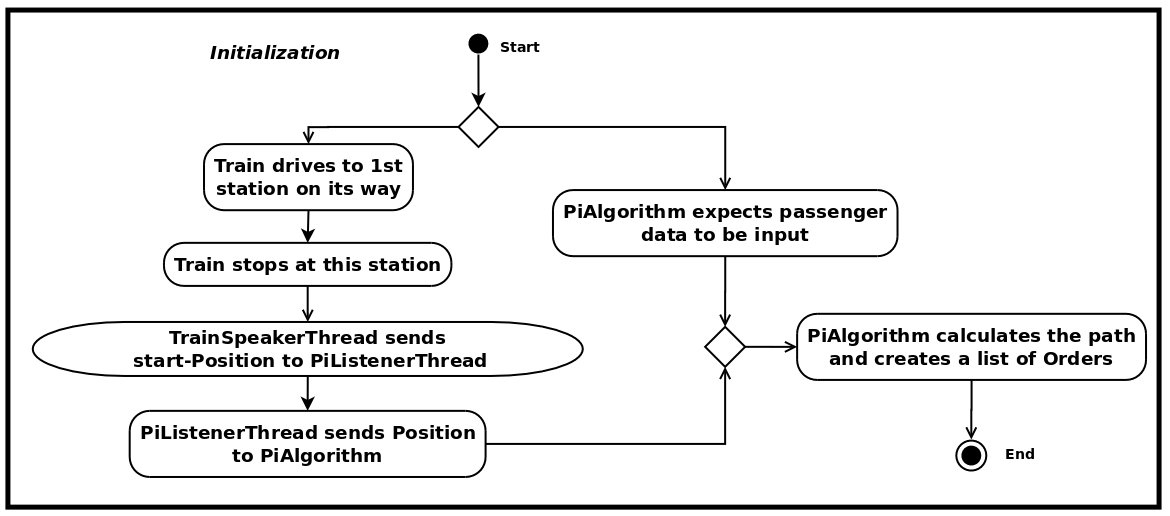
\includegraphics[width=2\textwidth, width=470pt]{content/images/Act-dia1.png}
\label{pic:init}
\end{figure}
%
\noindent
Im guten Szenario (so lange alle RFID-Tags vom Zug richtig erkannt werden) muss der Algorithmus die Liste von Anweisungen lediglich einmal erstellen; ansonsten wird die Methode \textit{repairOrderlist()} aufgerufen, die die createOrderlist()-Methode wieder verwendet und die neue Reihe von Anweisungen erstellt. Der Pi sendet mithilfe von PiSpeakerThread immer nur eine Anweisung und wartet, bis die geschickte Position (Tag) vom Zug erreicht und dem PiListenerThread mitgeteilt wird. Wenn sie übereinstimmen, ist alles in Ordnung und die nächste Anweisung kann geschickt werden, bis die Liste von Anweisungen leer wird.\\
\\
Das unten angegebene Diagramm stellt den Zusammenhang zwischen den Methoden und deren Reihenfolge grafisch dar. \\
\begin{figure}[H]	
\caption{Der gewöhnliche Verlauf}
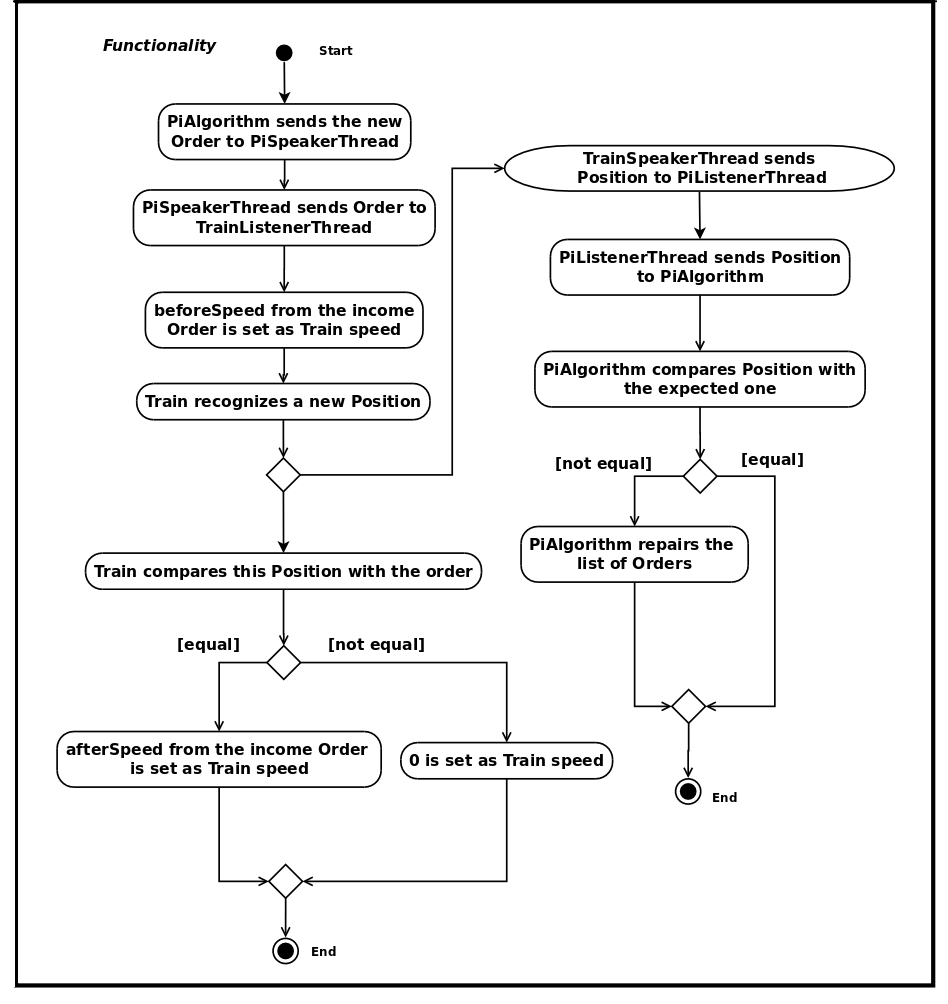
\includegraphics[width=2\textwidth, width=470pt]{content/images/Act-dia2.png}
\label{pic:init}
\end{figure}
%
\begin{figure}[H]	
\caption{Klassendiagramm}
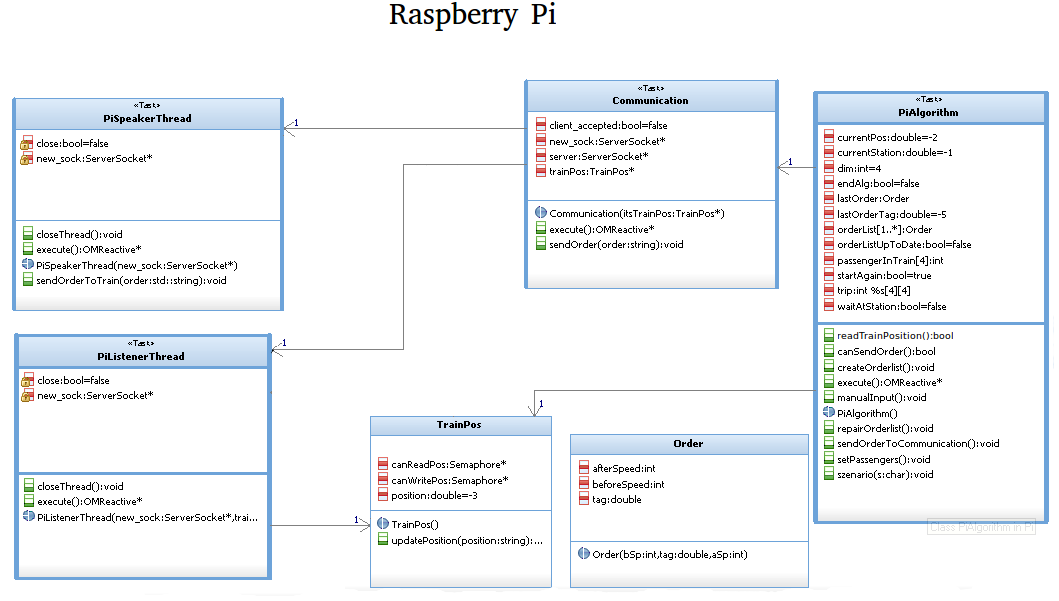
\includegraphics[width=2\textwidth, width=470pt]{content/images/RaspberryPi.png}
\label{pic:init}
\end{figure}
%
\section{createOrderList() - Methode}
Der Algorithmus wurde von uns komplett entwickelt. Die Hauptaufgabe des Algorithmus ist die Berechnung der Liste von Anweisungen. Sobald diese vorhanden ist, bleibt es lediglich, die Anweisungen aus der Liste eine nach der anderen dem Zug zu schicken, bis die Liste leer ist. Wenn die Liste leer geworden ist und die letzte Anweisung dem Zug geschickt wurde, hat der Raspberry Pi seine Arbeit gemacht. Er teilt das dem Nutzer mit und ist bereit, neue Aufgaben zu bekommen (neue Eingaben der Reisende aufzunehmen). Die Start-Position ist dem Zug bereits bekannt - dies ist die letzte Position, die der Zug dem Pi beim Erreichen der Endstation mitteilt. So kann man auf die Fahrt zum ersten Bahnhof, die der Zug immer nach dem Start des Systems gemacht hat, verzichten.\\
\\
Dabei sind folgende Bemerkungen wichtig:\\
\\
1) Die Matrix wird als ein zweidimensionaler Array implementiert.\\
\\
2) Die Einträge, die sich auf der Hauptdiagonale der Matrix befinden, sollen gleich 0 sein und ignoriert werden. In der Realität macht es keinen Sinn, Reisende zu haben, die vom Bahnhof 0 zum Bahnhof 0, d.h. einen vollen Kreis, fahren. In der \textit{createOrderlist()}-Methode werden solche Einträge deshalb ignoriert. Bei der Eingabe des Nutzers wird eine Meldung ausgegeben, falls ein Eintrag auf der Hauptdiagonale ungleich 0 ist, und ein solcher Eintrag wird auf 0 gesetzt - lediglich für die genaue Darstellung, denn diese Einträge werden gar nicht berücksichtigt.\\
\\
3) Die längste Strecke, die der Zug fahren kann, ist beim Start am Bahnhof 0 gleich einem vollen Kreis und danach bis zum Bahnhof 2 (genau 1.5 Kreise). Dies lässt sich folgend erklären: Alle Reisende, die Bahnhöfe 3 und 0 erreichen müssen, können das bereits beim ersten Kreis machen. Es bleiben Reisende, die vom Bahnhof 2 zum Bahnhof 1, und die vom Bahnhof 3 zu den Bahnhöfen 1 und 2 fahren müssen. Im allgemeinen (wichtig für die mögliche Vergrößerung der Anzahl von Stationen) fährt der Zug am längsten \textit{(einen vollen Kreis) + bis zu dem (N-2)-ten Bahnhof nach dem Start-Bahnhof,} wo N die Anzahl der Bahnhöfen darstellt. In unserem Fall (4 Bahnhöfe) entspricht das \textit{einem Kreis + bis zu dem (4-2)-ten (=2.ten) Bahnhof.}\\
\\
4) Die Anweisungen für die Zwischenhaltenstellen sind von den Anweisungen für die Bahnhöfe abhängig und lassen sich aus diesen erstellen. Beispiel aus dem Szenario 1: Der Zug startet am Bahnhof 0 und hält weiter an Bahnhöfen 1, 2 und 3. Danach fährt er allerdings am Bahnhof 0 durch. Dies bedeutet, der Zug kann an der Zwischenhaltestelle 3.5 schneller fahren.\\
\\
5) Der Algorithmus arbeitet mit der Dimension der Matrix \textit{dim=N} und ist somit flexibel - er kann auf eine Matrix beliebiger Größe eingesetzt werden.\\
\\
6) Die Hauptdiagonale der Matrix ist "flexibel" - dies ist für die Logik der \textit{createOrderlist()}-Methode wichtig. Aus Bequemlichkeit betrachten wir das Beispiel mit dem Start am Bahnhof 0. So sieht die Diagonale gewöhnlich aus. Bei einem Start, z.B., am Bahnhof 2, wird sie allerdings "versetzt" und somit folgendermaßen aussehen:\\
\\
\begin{figure}[H]	
\caption{Versetzung der Hauptdiagonale}
\center
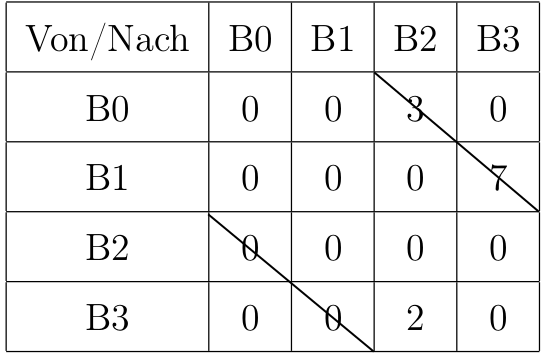
\includegraphics[width=2\textwidth, width=270pt]{content/images/matrix2.png}
\label{pic:DiagonaleVersetzt}
\end{figure}
\noindent
Damit man die Versetzung der Hauptdiagonale besser versteht, kann man sich die vorgenommene Transformation der Matrix folgend vorstellen: Die ersten zwei Zeilen werden ausgeschnitten und nach der Zeile "B3" hinzugefügt. So definiert die Startposition des Zuges immer die "pseudo-erste" Zeile der Matrix. Dabei werden die Elemente in der Matrix nicht unnötig kopiert - die Iteration durch die Matrix wird später lediglich anhand des Modulo-Operators angepasst. Aus Bequemlichkeit betrachten wir nun das Beispiel, in dem der Zug am Bahnhof 0 startet.\\
\\
\textit{\textbf{Wie erstellt der Algorithmus die Liste von Anweisungen?}\\}
\\
Dies lässt sich anhand der Matrix für das oben beschriebene Szenario 1 erklären.\\
\begin{figure}[H]	
\caption{Matrix mit einer Hauptdiagonale}
\center
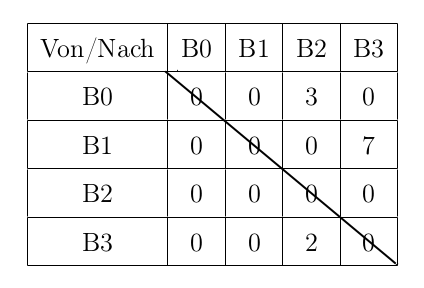
\includegraphics[width=2\textwidth, width=310pt]{content/images/matrix.png}
\label{pic:Hauptdiagonale}
\end{figure}
\noindent
Es wird ein Hilfsfeld \textit{stop} erstellt. Seine Länge ist (2*N - 2); es enthält boolesche Elemente, die mit "false" initialisiert werden. "False" entspricht dabei der Anweisung "do not stop", d.h. der Zug fährt an dem RFID-Tag weiter. Das erste Element (mit Index 0) im Feld \textit{stop} entspricht dabei dem Bahnhof, der gleich nach dem Start-Bahnhof kommt (in unserem Fall also dem Bahnhof 1), das zweite (Index 1) - dem weiteren Bahnhof (Bahnhof 2), usw. Das N-te Element (Index N-1) entspricht dem Start-Bahnhof, allerdings nach einem vollen Kreis. Deshalb muss man die beiden Hälften des Feldes unterschiedlich bearbeiten.\\
\\
Die Matrix wird dreimal durchgelaufen.\\
1) Beim 1. Durchlauf wird lediglich die "pseudo-erste" (in diesem Fall tatsächlich die erste) Zeile analysiert, nämlich die Zeile "B0". Alle Einträge, die ungleich 0 sind, verlangen vom Zug das Anhalten noch im ersten Kreis (genauer gesprochen, ist diese Strecke genau 1 Station kleiner, als ein voller Kreis) am Bahnhof, der dem Index der Spalte entspricht. In unserem Fall ist das Spalte "B2". Deshalb wird stop[1] gleich "true".\\
\\
2) Beim 2. Durchlauf (getrennt vom 1. Durchlauf nur für die Lesbarkeit, hat dasselbe Zweck und kann zusammengefasst werden) werden alle Einträge über der (pseudo-) Hauptdiagonale berücksichtigt. Die Zeile, die mindestens einen nicht leeren Eintrag hat, setzt das Element mit dem entsprechenden Index in \textit{stop} auf "true". In unserem Fall ist das die Zeile B1. Deshalb wird stop[0] gleich "true". Es wird auch stop[2] (entspricht Bahnhof 3) auf "true" gesetzt, da dies der Zielbahnhof der Reisende vom Bahnhof 1 ist. Die Spalte hat also den gleichen Einfluss.\\
\\
3) Beim 3. Durchlauf werden die Elemente unter der Hauptdiagonale berücksichtigt. Während die Durchläufe 1) und 2) immer für die Strecke \textit{(Vollkreis - 1 Station)} verantwortlich sind, erledigt der 3. Durchlauf die letzte Hälfte des Feldes \textit{stop}. So wird der Eintrag "2" in der Zeile "B3" dazu führen, dass das Element stop[2] (nochmal!) auf "true" gesetzt wird (allgemein notwendig, obwohl man am Bahnhof 3 schon anhält - ein Zufall dank dem Eintrag in der Zeile "B1", das wird nicht immer so sein). Außerdem wird stop[5] auf "true" gesetzt: Bahnhof "B2" muss erreicht werden.\\
\\
4) Nun muss man das letzte Element mit dem Wert "true" in \textit{stop} finden. Dies ist die Endstation des Zuges. Falls ein solches gar nicht vorhanden ist, hat der Zug laut der Eingabe des Nutzers nichts zu tun. In unserem Fall sieht das Feld \textit{stop} folgendermaßen aus:\\
\begin{figure}[H]	
\caption{Hilfsfeld \textit{stop}}
\center
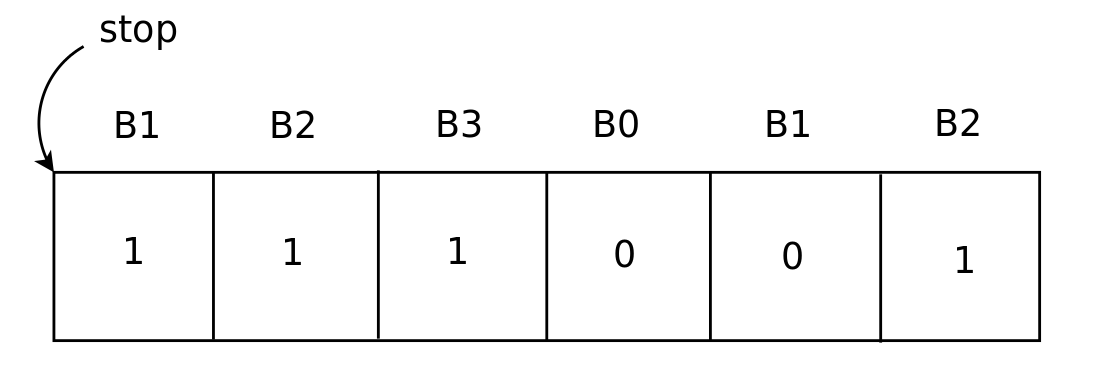
\includegraphics[width=2\textwidth, width=290pt]{content/images/stop1.png}
\label{pic:stop1}
\end{figure}
\noindent
5) Anhand der Einträge im Feld \textit{stop} kann man nun die Anweisungen erstellen. Nämlich werden für jedes Element (bis zu der Endstation) aus \textit{stop} zwei Anweisungen erstellt: Für die Zwischenhaltestelle und für den Bahnhof. Die Geschwindigkeiten sind folgend definiert: "low" (gleich 1), falls der Zug nach dem Anhalten vom Bahnhof erst startet oder nach der Zwischenhaltestelle an einem Bahnhof anhalten muss; "0", falls der Zug an dem RFID-Tag anhalten soll (dies macht nur bei \textit{afterSpeed} Sinn); ansonsten "high" (gleich 2), was einer hohen Geschwindigkeit entspricht. Die tatsächliche Geschwindigkeit wird auf der Zug-Seite definiert. So abstrahiert der Algorithmus von den technischen Details des Zuges und arbeitet nur mit für ihn verständlichen Geschwindigkeiten "schnell", "langsam", und "stehen bleiben".\\
\\
Eine grafische Darstellung der Liste mit Anweisungen \textit{orderList} findet man unten für das Hilfsfeld \textit{stop} für das zweite Szenario.\\
%to edit
\\
Im \textit{zweiten Szenario} möchten lediglich drei Reisende vom Bahnhof 0 zum Bahnhof 2 fahren.\\
\begin{table}[H]
\caption{Szenario 2}
\center
 \begin{tabular}{|c|c|c|c|c|}
 \hline
  Von/Nach & B0 & B1 & B2 & B3 \\ \hline
  B0 & 0 & 0 & 3 & 0\\   \hline
    B1 & 0 & 0 & 0 & 0 \\   \hline
      B2 & 0 & 0 & 0 & 0\\   \hline
        B3 & 0 & 0 & 0 & 0 \\   \hline
 \end{tabular}
\end{table}
\noindent
Damit die Aufgabe schwieriger wird und gleichzeitig um den oben genannten Ansatz zu erklären, werden wir als Start-Position den Bahnhof 1 betrachten.\\
\\
\begin{figure}[H]	
\caption{Szenario 2}
\center
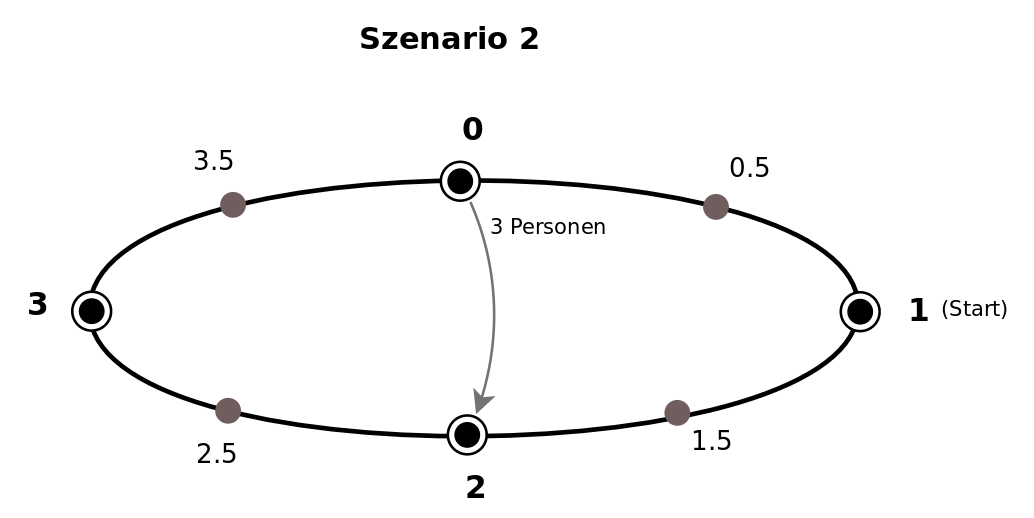
\includegraphics[width=2\textwidth, width=350pt]{content/images/szenario2.png}
\label{pic:szenario2}
\end{figure}
\noindent
Die Liste der Anweisungen \textit{orderList} und das Feld \textit{stop} sehen in diesem Fall folgendermaßen aus:\\
\begin{figure}[H]	
\caption{\textit{orderList} für Szenario 2}
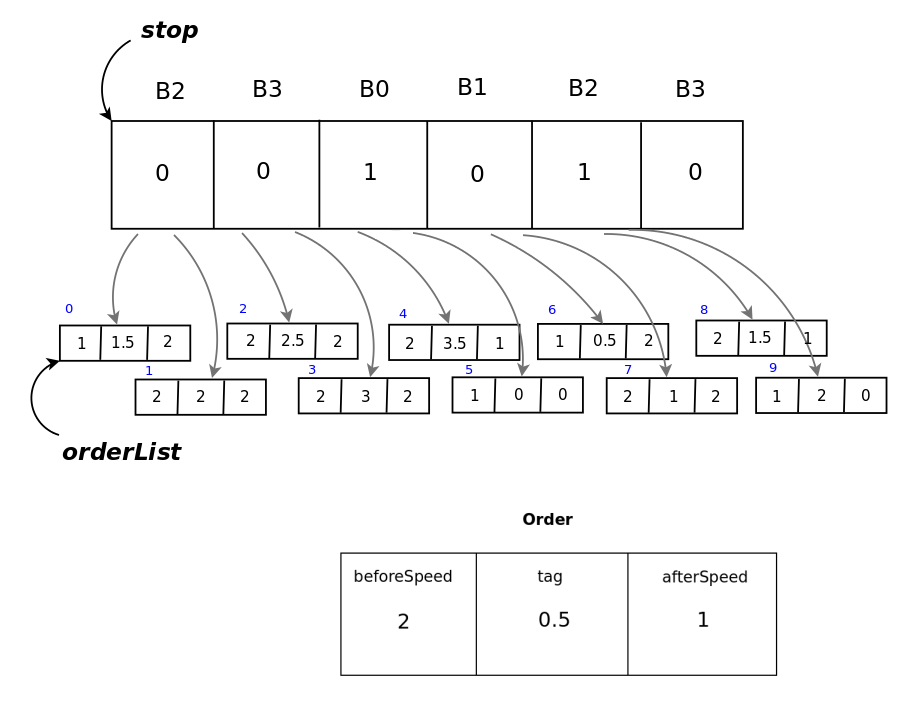
\includegraphics[width=2\textwidth, width=430pt]{content/images/orderList.png}
\label{pic:orderList2}
\end{figure}
\noindent
Man sieht aus den Anweisungen, dass der Zug langsam startet: Mit Geschwindigkeit "1" bis zum Tag "1.5". Dort setzt er sie auf "2" und fährt so bis zum Tag "3.5". Ab dort muss er langsamer fahren: Er kommt einem Bahnhof nah, bei dem er anhalten soll - Bahnhof 0. Dort steigen Reisende ein und der Zug fährt langsam ab. Beim Tag "0.5" darf er wieder schneller werden und fährt deshalb mit "2" bis zum Tag "1.5", wo er wieder langsamer (\textit{afterSpeed} gleich "1") wird. Am Tag "2" bleibt der Zug stehen - dies ist seine Endstation.\\
\section{Laufzeit und alternative Ansätze für die Implementierung}
%Laufzeit
Die \textbf{\textit{Laufzeit des Algorithmus}} ist folgendermaßen definiert:\\
$T = O( (n-1) + (n-1)*(n/2) + (n-1)*(n/2) ) = O(n^2)$\\
\\
Dabei wurde von den Entwicklern überlegt und diskutiert, ob der Algorithmus am Anfang die Route komplett berechnen und erst dann die erste Anweisung dem Zug schicken soll oder jedes Mal, wenn die Position des Zuges ihm mitgeteilt wurde überprüfen soll, was der Zug als nächstes zu tun hat. Es wurde die erste Variante gewählt und implementiert, welche als Vorteil die Eigenschaft hat, dass der Algorithmus ohne Verzögerung, die für die Berechnung notwendig ist, die nächste Anweisung dem Zug mitteilen kann. Als Kritik kann man den Punkt nennen, dass die Verzögerung am Anfang sich sammelt und dadurch größer ist. Außerdem soll die zweite Variante genommen werden, falls man häufige Änderungen (neue Eingaben der Reisende) erwartet. Diese Überlegungen sind allerdings nur für sehr große Dimensionen der Matrix wichtig und haben somit für die Geschwindigkeit in diesem Projekt keine Relevanz.\\
\\
Darüber hinaus wurde diskutiert, ob man zusätzlich zu der Matrix bzw. an ihrer Stelle eine verkettete Liste verweden könnte. Dies scheint den Algorithmus in dem Fall, dass der Zug auch im inneren Kreis fahren können soll, zu vereinfachen. So sind in diesem Fall an bestimmten Stellen Verzweigungen der Strecke möglich. Allerdings ist die Matrix lediglich eine Art der Darstellung von den Eingaben des Nutzers und lässt sich weiter beliebig anpassen und bearbeiten. So könnte man zwei weitere Zeilen B4 und B5 hinzufügen und vereinbaren, dass es vom Bahnhof 0 sowohl zum Bahnhof 1 (Zeile B1), als auch zum Bahnhof 5 (Zeile B5) einen Weg gibt.\\
%
%
\section{repairOrderList() - Methode}
Es kann passieren, dass der Zug einen RFID-Tag überfährt, ohne ihn zu erkennen. Der Zug wird in diesem Fall einen "falschen" Tag lesen und dem Algorithmus diesen Tag mitteilen, während er selbst nicht weiter fährt (ein Sicherheitsmechanismus). Der Algorithmus muss diese Abweichung behandeln. Dafür wird im Zug ein Buch über die Reisende geführt, die sich gerade im Zug befinden, zusammen mit ihren gewünschten Zielbahnhöfen. Wenn Reisende in den Zug einsteigen, werden sie aus der Matrix gelöscht. Wenn die Reisende aus dem Zug aussteigen, werden sie auch aus dem Buch im Zug gelöscht. So kann man bei einer Abweichung immer erkennen, wer noch an Stationen wartet und wer sich im Zug befindet (und wo er oder sie hin möchte). Eine neue Ausführung der Methode \textit{createOrderlist()} "repariert" die Liste mit Anweisungen. Dies ist nicht immer notwendig: Vielleicht hat der Zug eine Zwischenhaltestelle nicht erkannt und dort nicht langsamer bzw. schneller geworden?. Oder der Zug ist an Stationen vorbei gefahren, wo er nicht anhalten musste? In diesem Fall muss man eine neue Liste nicht erstellen, sondern man muss nur eine bzw. einige Anweisungen (die schon jedenfalls zufällig vom Zug durch Vorbeifahren ausgeführt wurden) aus der Liste entfernen, ohne diese dem Zug zu schicken. Die \textit{repairOrderlist()}-Methode kann somit verbessert werden. Bei unserer Anzahl der Bahnhöfe ist das unwichtig; bei einer großen Matrix lässt sich die Rechenzeit somit sparen.\\
%
%
%
%\begin{figure}[H]	
%\caption{...}
%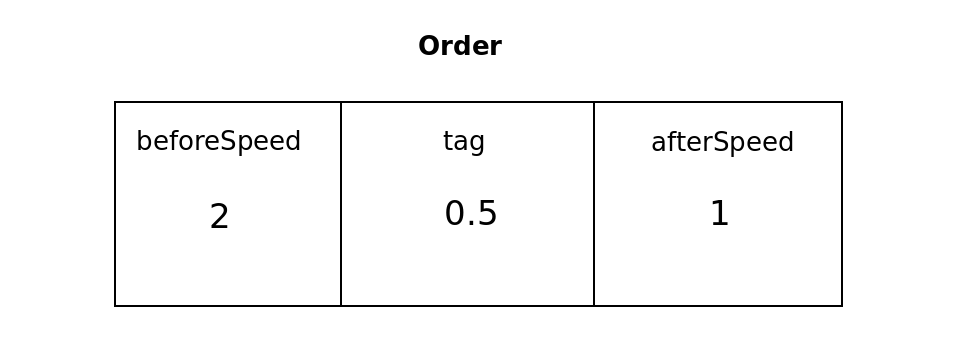
\includegraphics[width=2\textwidth, width=470pt]{content/images/order.png}
%\label{pic:pi_communication}
%\end{figure}
%
\chapter{Semaphore}
Die Semaphore und ihr Einsatz werden anhand der Implementierung an der Pi-Seite erklärt.\\
\\
Nachdem der Algorithmus die Eingaben des Nutzers gespeichert hat, braucht er die Start-Position des Zuges, damit er die Liste von Anweisungen erstellen kann. Diese erfährt er mithilfe von der Methode \textit{readTrainPosition()}. Der Wert darf allerdings erst dann gelesen werden, wenn der Zug ihn dem PiListenerThread mitgeteilt hat. Bevor das passiert, darf der Algorithmus nichts machen und muss blockiert sein. Die einfache Lösung, die sich anbieten könnte, besteht darin, dass man eine weitere Methode \textit{algorithmCanRead()} hinzufügt, die ein "Flag" - eine boolesche Variable - überprüft, die vom PiListenerThread auf "erlaubt" gesetzt wird, sobald die Position aktualisiert wurde. Der Algorithmus liest die Position und setzt das "Flag" selbst auf "nicht erlaubt" - damit er sie nicht wieder liest, bevor eine neue Position vom Zug mitgeteilt worden ist. Das Wort "blockiert" ist hier entscheidend. Wie oft soll das "Flag" überprüft werden? Wie lange soll der Algorithmus blockiert werden? Wie bekommt er rechtzeitig mit, dass die Position aktualisiert wurde? Der oben genannte Ansatz verlängt Polling, d.h. Ressourcen(Rechenzeit)-Verschwendung. Die richtige Lösung an dieser Stelle ist der Einsatz von Semaphoren.\\
\\
Rhapsody bietet eine Factory von Semaphoren an. Ein Factory-Objekt verfügt über eine Methode \textit{createOMOSSemaphore()}, die den Zeiger auf eine neuerstellte Semaphore zurückliefert. Bei der Erzeugung kann man definieren, ob die Semaphore frei ist oder blockieren soll (das Attribut \textit{initialCount}, by default gleich 1) und wie groß der maximale Wert (das Attribut \textit{maxCount}, bezeichnet die Anzahl von Ressourcen, by default auch 1) sein soll. Die Semaphore bietet die Methoden \textit{p()} (Ressource nehmen) und \textit{v()} (Ressource freigeben), die hier \textit{wait(-1)} und \textit{signal()} genannt werden. Wenn ein Thread \textit{wait(-1)} aufruft, während \textit{initialCount} den Wert 0 hat (keine Ressourcen vorhanden), wird er blockiert. \textit{Signal}() blockiert, wenn \textit{initialCount} gleich \textit{maxCount} ist, allerdings nicht bei allen Plattformen.\\
In unserem Fall ist es wichtig, dass signal() auch blockiert, denn wir wollen nicht, dass der PiListenerThread die Position des Zuges aktualisiert, bevor der Algorithmus (der aus irgendwelchem Grund zu langsam war) die alte Position einmal gelesen hat. Dies würde dazu führen, dass der Algorithmus nicht mitbekommt, dass der Zug da war, wo er sein musste, und dass der Zug seine Position richtig erkannt hat, und es wird \textit{repairOrderlist}()-Methode aufgerufen.\\
\\
Wir wollen von OMOSSemaphoren abstrahieren und erstellen deshalb eine eigene Klasse Semaphore, die Methoden \textit{request()} (die bekannte Methode p() ) und \textit{release()} (die Methode r() ) enthält. Wir brauchen zwei Objekte (bzw. Zeiger) dieser Klasse, die in der Klasse \textit{TrainPos} als Attribute vorhanden sind: \textit{canReadPos} und \textit{canWritePos}.\\
\\
\textit{canReadPos} ist am Anfang blockiert, falls der Algorithmus \textit{request}() aufruft: Man darf noch nicht lesen. Der Zug teilt seine Position mit und der PiListenerThread aktualisiert sie (\textit{canWritePos} erlaubt ihm, \textit{request}() aufzurufen), zusätzlich ruft er \textit{release}() für \textit{canReadPos}. Nun wäre PiListenerThread blockiert, falls er gleich wieder \textit{request}() für \textit{canWritePos} aufruft. Er muss warten, bis der Algorithmus die Position einmal gelesen und \textit{release}() für \textit{canWritePos} aufgerufen hat.\\
\\
Aus dieser Beschreibung des gewünschten Verlaufs ist es klar, dass wir die Semaphore \textit{canReadPos} und \textit{canWritePos} folgend initialisieren müssen: (initialCount=0, maxCount=1) für den ersten und (initialCount=1, maxCount=1) für den zweiten.\\
%\end{document}
\chapter{Zug}
\section{Funktionsweise}

Aufgrund der Verlagerung der Logik auf den Raspberry Pi ist die Funktionsweise des Zuges sehr beschränkt.\\
Beim Start der Zugsoftware wird zuerst eine langsame Fahrt des Zuges durchgeführt um mithilfe des als nächstes gelesenen Tag die Position des Zuges zu bestimmen. Diese wird nun an den Raspberry Pi übermittelt und die Antwort abgewartet. Die nun empfangene Anweisung wird durchgeführt, was bedeutet das die Werte für "beforeSpeed", "tag" und "afterSpeed" ausgelesen und abgespeichert werden. "beforeSpeed" wird zusätzlich als aktuelle Geschwindigkeit gesetzt.\\
Wird nun während der Ausführung der Anweisung ein neuer Tag gelesen wird dieser mit dem Wert aus "tag" verglichen. Sollte sich der gelesene Tag von dem gespeicherten unterscheiden hält der Zug an. Ansonsten wird "afterSpeed" als neue Geschwindigkeit gesetzt. In jedem Fall wird der gelesene Tag erneut an den Raspberry Pi übermittelt.\\
Abgesehen von der Socket-Verbindung (Beschrieben in Kapitel \ref{chap:socket}) wurde keine weitere Logik für den Zug implementiert.

\section{Merging der Projekte in ein Projekt}
\begin{figure}
	\caption{Aufbau der Projekte. Rechts das alte, links das neue Projekt}
	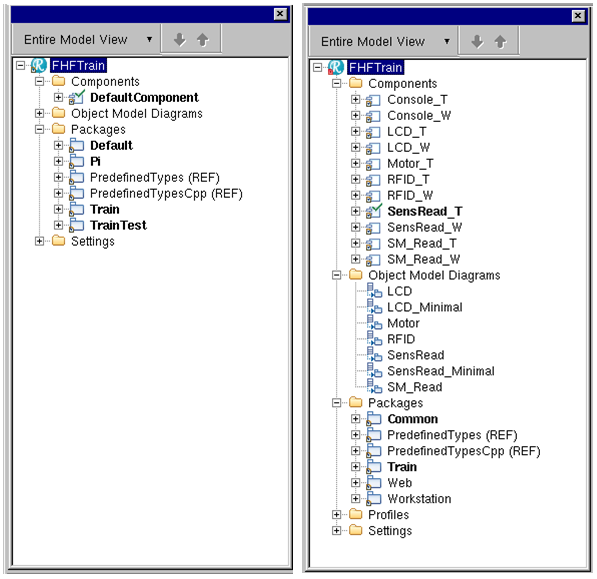
\includegraphics[width=1\textwidth]{content/pictures/train/structure.png}
	\label{pic:train_structure}
\end{figure}
Das FHFTrain-Projekt basiert auf dem Semesterprojekt des Sommersemesters 2016. Der Code, der den Zug grundsätzlich zum Fahren bringt und die Hardware ansteuert, muss also zusammen mit dem neuen Code, also Algorithmus und Socket, "gemerged" werden. In Abbildung \ref{pic:train_structure} sieht man zunächst den jeweils grundgelegenen Aufbau der beiden Projekte.\\  
Das alte Semesterprojekt beinhaltet mehrere Components, die jeweils mit T oder W beschriftet sind, für Train und Workstation.\\
Das aktuelle Projekt beinhaltet nur eine Component und mehreren Packages, jeweils für den Raspberry Pi (Als Pi bezeichnet) und den Zug (Als Train bezeichnet). Zusätzlich gibt es noch ein Testpackage, TrainTest.\\
Zunächst wird das alte Projekt geöffnet, über \textit{File->Insert Project->Existing…} lässt sich ein zweites Projekt in die Modelübersicht aufnehmen. Danach können sowohl Components, als auch Diagramme und Packages per \textit{Ctrl+Drag} übertragen werden. In der finalen Version wird die "DefaultComponent" aus dem aktuellen Projekt in die Components "Algorithm\_Socket" und "Train\_Socket" aufgeteilt. "Algorithm\_Socket" verwaltet dabei den kompletten Algorithmus und die Socket-Verbindung auf dem Pi. "Train\_Socket" hingegen ist für die Kommunikation auf dem Zug zuständig, diese Component verwaltet also, was an den Pi geschickt wird und wie die Informationen gehandhabt werden sollen, die vom Pi ankommen.\\
In Abbildung \ref{pic:train_structure_merged} ist die vollständige Modellübersicht des gemergten Projektes zu sehen.
\begin{figure}
	\caption{Aufbau des Projektes nach dem Merge}
	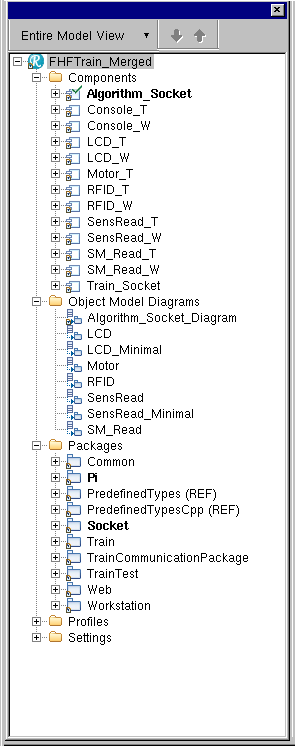
\includegraphics[height=0.8\textheight]{content/pictures/train/structure_merged.png}
	\label{pic:train_structure_merged}
\end{figure}

\section{Zusammenführung des Codes}

Nachdem beide Projekte „gemerged“ worden sind, müssen noch mehrere Stellen im Code modifiziert werden.\\
Im ersten Schritt wird eine Verbindung zwischen der Train-Kommunikation und der Shared-Memory aufgebaut. Die Shared-Memory steht allen Komponenten des Zuges zur Verfügung, über diese können die Komponenten Daten austauschen. In der Shared-Memory werden Datentypen für AfterSpeed und BeforeSpeed erstellt, also die Geschwindigkeiten, die der Zug bis zu einem Tag und ab einem Tag fahren soll.\\
Als nächstes wird eine Methode implementiert, die die Befehle des Pis in Substrings unterteilen und die Geschwindigkeiten in die Shared-Memory eintragen. Die Motor-Komponente sorgt dann automatisch dafür, dass die neue Geschwindigkeit gefahren wird.\\
Im letzten Schritt muss noch dafür gesorgt werden, dass der Zug dem Pi auch seine Position mitteilen kann. Dazu wird eine Funktion implementiert, die immer, wenn der Zug einen RFID Tag erkennt, einen dazugehörigen float-Wert in die Shared-Memory speichert. Schließlich wird noch implementiert, dass der TrainSpeaker genau dann seine Position an den Pi sendet, wenn in der Shared-Memory eine Änderung des RFID-Tags stattgefunden hat.\\
Nach diesen Arbeitsschritten sind die beiden Projekte endgültig  zu einem Projekt „gemerged“, welches dann auch funktionstüchtig ist.

\chapter{Socket}
\chapter{Tests}
\chapter{Buildprozess}

\section{Zug}

\section{Raspberry Pi}


% Beispielkapitel  %alle von EG auskommentiert
%\chapter{Einleitung}

\section{Strukturen}

\subsection{asdasd}
asdfasdf

\subsubsection{Subsubsection}
asdf

\paragraph{Paragraph}
asdf

\section{Beispielabbildungen}

\lipsum[10]

\begin{wrapfigure}{rt}{8cm}
\caption{Bildüberschrift}
\centering

\includegraphics[width=0.3\textwidth]{content/pictures/hfu}
Quelle: \cite{s11wasml}
\label{pic:bild2}
\end{wrapfigure}

\lipsum[10]

\begin{figure}
\caption{Bildüberschrift}

\includegraphics[width=1\textwidth]{content/pictures/hfu}
Quelle: \cite{s11wasml}
\label{pic:bild1}
\end{figure}

\section{Beispieltabelle}

\begin{table}
\caption{Tabellenüberschrift}
\center
\footnotesize
\begin{tabular}{lll}
\toprule
Head1 & Head2 & Head3 \\
\midrule
Val1 & Val2 & Val3 \\
Val4 & Val5 & Val6 \\
\bottomrule
\end{tabular}
\end{table}

\section{Listings}

\begin{lstlisting}[language=java, caption=Hallo Welt in Java]
public class HalloWelt 
{
	public static void main(String[] args) 
	{
		System.out.println("Hallo Welt!");
	}
}
\end{lstlisting}

\section{Abkürzungen}

Im Abkürzungsverzeichnis stehende Abkürzungen können in Langform (\ac{HFU}) oder in Kurzform (\acs{HFU}) angegeben werden.

\section{Abgesetztes wörtliches Zitat}

\lipsum[10]

\begin{quote}
\textit{\enquote{Eingerücktes wörtliches Zitat.}}\cite[S. 14ff]{s11wasml}
\end{quote}

\lipsum[10]

\section{Theoreme}

\lipsum[2]

\begin{beispiel}
Beispieltext\dots
\end{beispiel}
 
\lipsum[2]

\begin{these}
These\dots
\end{these}
 
\lipsum[2]
 
\begin{definition}
Unter dem Begriff \dots verstehen wir \dots
\end{definition}

\lipsum[2]
%\chapter{Grundlagen}
\begin{figure}
\caption{Bildüberschrift}

\includegraphics[width=1\textwidth]{content/pictures/hfu}
\label{pic:bild3}
\end{figure}
%\chapter{[Eigene Kapitel]}
%\chapter{Ausblick}
%\chapter{Fazit}

% Schalgwortverzeichnis (Index)
%\printindex

% Literaturverzeichnis
\singlespacing
\bibliographystyle{alphadin}
\bibliography{bibtex}

% Eidesstattliche Erklärung
\chapter*{Eidesstattliche Erklärung\markboth{Eidesstattliche Erklärung}{}}
% Eintrag in das Inhaltsverzeichnis 
\addcontentsline{toc}{chapter}{Eidesstattliche Erklärung}

Ich versichere, dass ich die vorstehende Arbeit selbständig verfasst und hierzu
keine anderen als die angegebenen Hilfsmittel verwendet habe. Alle Stellen der Arbeit die 
wörtlich oder sinngemäß aus fremden Quellen entnommen wurden, sind als solche kenntlich gemacht.
\\
\\
Die Arbeit wurde bisher in gleicher oder ähnlicher Form in keinem anderen
Studiengang als Prüfungsleistung vorgelegt oder an anderer Stelle
veröffentlicht.
\\
\\
Ich bin mir bewusst, dass eine falsche Erklärung rechtliche Folgen haben kann.

\vspace*{1.5cm} \par
\line(1,0){200} \par
\docOrt, den  \docAbgabedatum ~~\docVorname~\docNachname

\appendix
% Hier können Anhaenge angefuegt werden

\end{document}      